\documentclass[12pt]{article}
\usepackage[a4paper, total={6in, 8.5in}]{geometry}
\usepackage{graphicx}
\graphicspath{ {images/output/} }
\usepackage{amsmath}
\usepackage{minted}
\usepackage{multicol}
\usepackage{caption}
\usepackage[english]{babel}
\usepackage{placeins}
\usepackage{titling}


\begin{document}
\vspace*{\fill}
\begin{center}

    \emph{Heaven's Light is Our Guide} \\
    \textbf{Rajshahi University of Engineering and Technology} \\

    \begin{figure}[H]
        \centering
        
\includegraphics[scale=.34]{images/RUET_logo.png}
        \label{fig:ruet_logo}
    \end{figure}
    \vspace{5mm}

    \textbf{Course Code}\\
    ECE 2214\\
    \vspace{3mm}
    \textbf{Course Title}\\
    Numerical Methods and Discrete Mathematics Sessional

    \vspace{5mm}
    \textbf{Experiment Date:} {November 18, 2023},\\
    \textbf{Submission Date:} {December 2, 2023}\\

    \vspace{5mm}
    \textbf{Lab Report 10:} Implementing Secant method of root finding in MATLAB.

    \vspace{15mm}

    \begin{tabular}{c|c}
        \textbf{Submitted to} & \textbf{Submitted by} \\
        Md. Omaer Faruq Goni  & Md. Tajim An Noor     \\
        Lecturer              & Roll: 2010025         \\
        Dept of ECE, Ruet     &                       \\
    \end{tabular}

\end{center}
\vspace*{\fill}

\clearpage
\title{Implementing \& Plotting Taylor Series for Sine in MATLAB}
\author{}
\date{}
\maketitle

\section*{Introduction}
\subsection*{Taylor Series}
The Taylor series is a way to represent a function as an infinite sum of terms calculated from the values of the function's derivatives at a specific point.\\\\
For a function \(f(x)\) that is infinitely differentiable at a point \(a\), the Taylor series expansion around \(a\) is given by:
\[f(x) = f(a) + f'(a)(x-a) + \frac{f''(a)}{2!}(x-a)^2 + \frac{f'''(a)}{3!}(x-a)^3 + \ldots
\]
For sine function, the taylor series is expanded as:
\[\sin(x) = x - \frac{x^3}{3!} + \frac{x^5}{5!} - \frac{x^7}{7!} + \ldots\]

\section*{Tools Used}
\begin{itemize}
    \item MATLAB R2021a - for writing and running code.
    \item MacTeX -\LaTeX  compiler.
    \item VS Code with \LaTeX workshop extension as a text editor.
\end{itemize}

\section*{Process}
\subsection*{Code for Taylor sine series:}
\begin{minted}[breaklines, linenos]{matlab}
    close all;
    clear all;
    clc;
    syms x;
    f =input('Enter the function : ');

    theta = -pi:pi/20:pi;

    g = f;

    %hold on;
    y = input('Enter the value for approximation: ');
    a = input('Enter the starting point: ');

    n = input('Enter the number of order: ');

    taylor = eval(subs(f,x,a));

    for i = 1:n
        f = diff(f,x);
        taylor = taylor + ( eval(subs(f,x,a)) * power((x-a),i) / factorial(i) );
        disp(taylor);
        plot(theta,subs(taylor,x,theta));
        hold on;
        if i == n
        plot(theta,subs(g,x,theta));
        end
    end

    disp(eval(subs(taylor,x,y)));
\end{minted}
\subsection*{Output}
\begin{center}
    \centering
    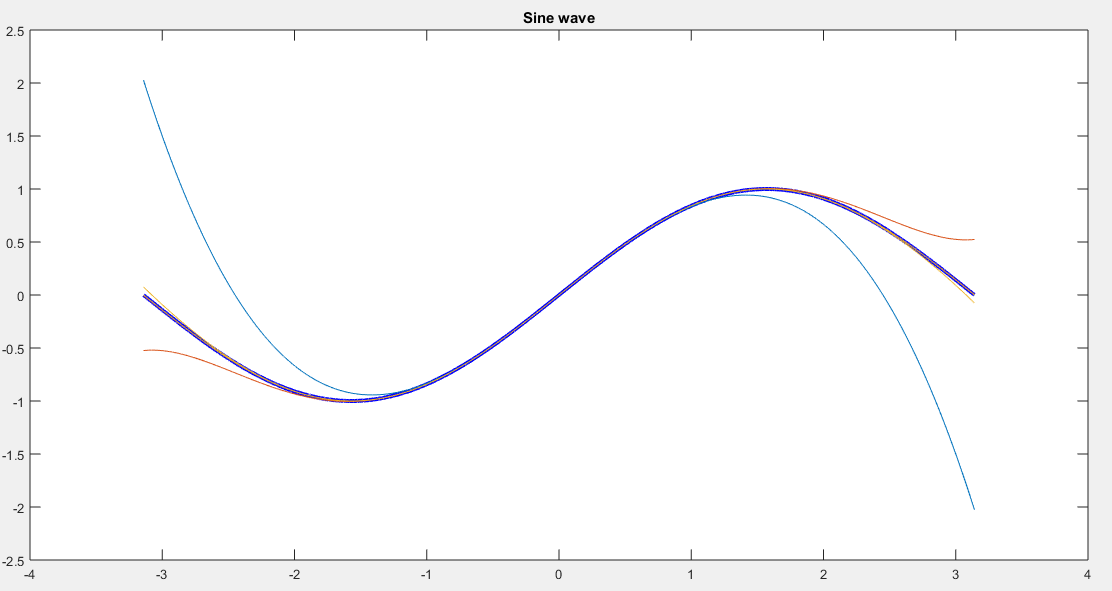
\includegraphics[width = .9\textwidth]{tay.png}
    \captionof{figure}{Taylor Sine Series ($-\pi \leq \:\: $x$ \:\: \leq \pi$)}
\end{center}




\clearpage
\title{Implementing Interpolation; Newton's Forward Method in MATLAB }
\author{}
\date{}
\maketitle

\section*{Introduction}
\subsection*{Interpolation, Newton's Forward Method}
Newton's Forward Interpolation is a numerical technique used for interpolating or estimating the value of a function between given data points. It belongs to the category of polynomial interpolation methods and is particularly useful when dealing with equally spaced data points.
\\\\
The method involves constructing a polynomial of degree \(n\) that passes through \(n+1\) equally spaced data points. It approximates the value of the function at an intermediate point within the range of the given data.
The general form of the Newton's Forward Interpolation polynomial is:
\[f(x) = P_n(x) = f(x_0) + \Delta y_0 \cdot P_1(u) + \Delta^2 y_0 \cdot P_2(u) + \ldots\]
Here, \(P_n(x)\) is the polynomial of degree \(n\) used for interpolation, \(f(x_0)\) represents the value of the function at the starting point \(x_0\), \(\Delta y_0\) denotes the first forward difference, \(\Delta^2 y_0\) signifies the second forward difference, and so on. The symbol \(u\) typically represents the normalized difference ratio \(\frac{x - x_0}{h}\), where \(h\) is the common difference between the data points.\\\\


\section*{Tools Used}
\begin{itemize}
    \item MATLAB R2021a - for writing and running code.
    \item MacTeX -\LaTeX  compiler.
    \item VS Code with \LaTeX workshop extension as a text editor.
\end{itemize}

\section*{Process}

\subsection*{Code for Newton's Forward Interpolation:}
\begin{minted}[breaklines, linenos]{matlab}
    clc;
    clear all;
    close all;
    matrix = [];
    
    number = input('How many pair of data is given: ');
    
    for i = 1:number
            matrix(i,1) = input('Enter value(x) : ');
            matrix(i,2) = input('Enter value(y) : ');
    end
    
    xo = matrix(1,1);
    xn = matrix(number,1);
    h = matrix(2,1)-xo;
    x = input('Enter the value for which the function is to be evaluated:');
    n = number -1;
    
    for j = 3: (number+1)
        for i = 1:n
            matrix(i,j) = matrix(i+1,j-1)-matrix(i,j-1);
        end
        n = n-1;
    end
    disp(matrix)
    p = (x-xo)/h;
    z = p;
    c = 3;
    y0 = matrix(1,2);
    for i = 1:number-1
        fprintf('y0 = %f + (%f * %f)/%d! \n',y0,p,matrix(1,c),i)
        y0 = y0 + (pmatrix(1,c))/factorial(i);
        c = c+1;
        p = p(z-i);
    end
    disp(y0);
\end{minted}

\subsection*{Output}
\begin{center}
    \centering
    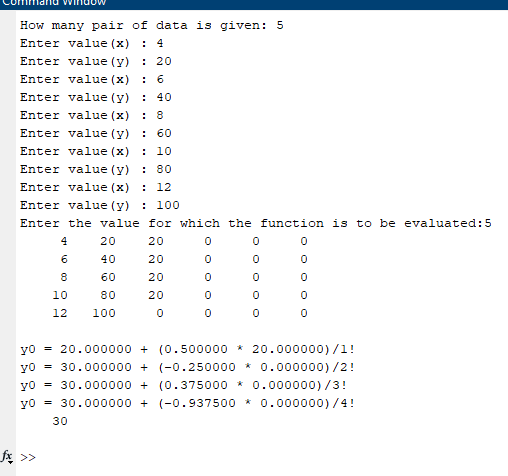
\includegraphics[width = .9\textwidth]{fwd.png}
    \captionof{figure}{Newton's Forward Method}
\end{center}
\clearpage
\title{Implementing Interpolation; Newton's Backward Method in MATLAB }
\author{}
\date{}
\maketitle

\section*{Introduction}
\subsection*{Interpolation, Newton's Backward Method}
Newton's Backward Interpolation is another numerical technique used for estimating the value of a function between given data points. Similar to Newton's Forward Interpolation, it falls under the category of polynomial interpolation methods and is particularly useful for equally spaced data points.\\\\
The general form of the Newton's Backward Interpolation polynomial is:
\[f(x) = P_n(x) = f(x_n) + \Delta y_{n-1} \cdot P_1(u) + \Delta^2 y_{n-2} \cdot P_2(u) + \ldots\]
Here, \(P_n(x)\) is the polynomial of degree \(n\) used for interpolation, \(f(x_n)\) represents the value of the function at the last point \(x_n\), \(\Delta y_{n-1}\) denotes the first backward difference, \(\Delta^2 y_{n-2}\) signifies the second backward difference, and so on. The symbol \(u\) typically represents the normalized difference ratio \(\frac{x - x_n}{h}\), where \(h\) is the common difference between the data points.


\section*{Tools Used}
\begin{itemize}
    \item MATLAB R2021a - for writing and running code.
    \item MacTeX -\LaTeX  compiler.
    \item VS Code with \LaTeX workshop extension as a text editor.
\end{itemize}

\section*{Process}

\subsection*{Code for Newton's Backward Interpolation:}
\begin{minted}[breaklines, linenos]{matlab}

\end{minted}

\subsection*{Output}
\begin{center}
    \centering
    % 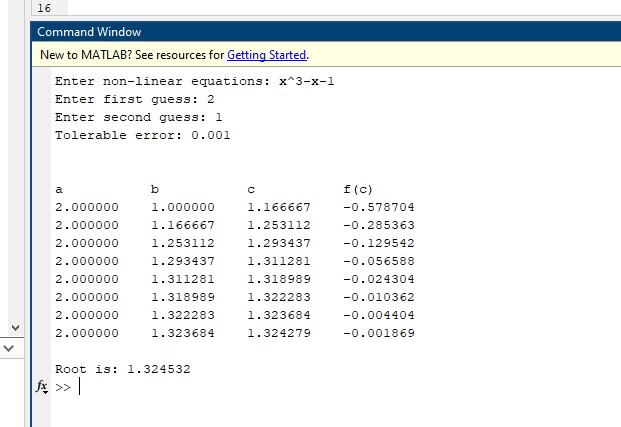
\includegraphics[width = .9\textwidth]{false.jpeg}
    \captionof{figure}{Newton's Backward Method}
\end{center}
\pagebreak
\section*{Functions}
The functions used to do the three methods in MATLAB are as such with brief description of each of them:
\begin{description}
    \item[]
\end{description}
These function are the newly learned ones for these experiments.
% \cite{matlab}
\pagebreak
\bibliographystyle{IEEEtran}
\bibliography{ref}

\end{document}
